\documentclass[tikz,border=4pt]{standalone}
\usepackage{amsmath}
\usetikzlibrary{arrows.meta}

\definecolor{teal}{RGB}{0,166,138}
\definecolor{meshfill}{RGB}{237,247,243}

\begin{document}
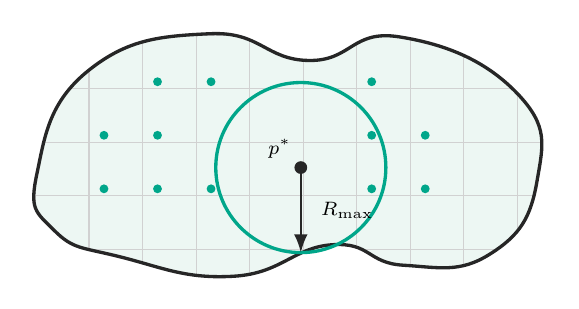
\begin{tikzpicture}[line cap=round,line join=round,>=Latex,font=\scriptsize]
  \path
    plot[smooth cycle,tension=.82] coordinates {
      (0.70,1.65) (1.35,2.95) (2.90,3.42) (4.15,3.08)
      (5.30,3.38) (6.80,2.66) (7.05,1.55) (6.45,.62)
      (5.35,.48) (4.45,.74) (3.20,.34) (1.78,.58) (.92,.92)};

  \fill[meshfill]
    plot[smooth cycle,tension=.82] coordinates {
      (0.70,1.65) (1.35,2.95) (2.90,3.42) (4.15,3.08)
      (5.30,3.38) (6.80,2.66) (7.05,1.55) (6.45,.62)
      (5.35,.48) (4.45,.74) (3.20,.34) (1.78,.58) (.92,.92)};

  \begin{scope}
    \clip plot[smooth cycle,tension=.82] coordinates {
      (0.70,1.65) (1.35,2.95) (2.90,3.42) (4.15,3.08)
      (5.30,3.38) (6.80,2.66) (7.05,1.55) (6.45,.62)
      (5.35,.48) (4.45,.74) (3.20,.34) (1.78,.58) (.92,.92)};
    \draw[black!18,step=.68] (.4,.2) grid (7.3,3.7);
    \foreach \x/\y in {1.55/1.45,2.23/1.45,2.91/1.45,4.95/1.45,5.63/1.45,1.55/2.13,2.23/2.13,4.95/2.13,5.63/2.13,2.23/2.81,2.91/2.81,4.95/2.81}
      \fill[teal] (\x,\y) circle (1.6pt);
  \end{scope}

  \draw[black!85,very thick]
    plot[smooth cycle,tension=.82] coordinates {
      (0.70,1.65) (1.35,2.95) (2.90,3.42) (4.15,3.08)
      (5.30,3.38) (6.80,2.66) (7.05,1.55) (6.45,.62)
      (5.35,.48) (4.45,.74) (3.20,.34) (1.78,.58) (.92,.92)};

  \coordinate (Seed) at (4.05,1.72);
  \draw[teal,very thick] (Seed) circle (1.08);
  \fill[black!85] (Seed) circle (2.3pt);
  \draw[black!85,thick,->] (Seed) -- (4.05,.64);
  \node[above left] at (Seed) {$p^*$};
  \node[right] at (4.18,1.18) {$R_{\max}$};
\end{tikzpicture}
\end{document}
